\pdfoutput=1
\documentclass[11pt]{article}

% Final version (the "review" option would anonymise authors and add line numbers).
\usepackage{EACL2023}

\usepackage{times}
\usepackage{latexsym}
\usepackage[T1]{fontenc}
\usepackage[utf8]{inputenc}
\usepackage{microtype}
\usepackage{inconsolata}
\usepackage{booktabs}
\usepackage{graphicx}
\usepackage{amsmath}
\usepackage{amssymb}
\usepackage{amsthm}
\usepackage{tikz}
\usetikzlibrary{positioning,arrows.meta}
\usepackage{pgfplots}
\pgfplotsset{compat=1.17}

\newtheorem{lemma}{Lemma}
\newcommand{\Cd}{C_{\mathrm{desc}}}
\newcommand{\wtl}[3]{#1/#2/#3}

\title{Noise in Disguise: What Powers\\
       Physics-Inspired GNN Colouring}

\author{Semyon Guretskiy \\ 336249255 \And
        Ori Petel \\ 325211498 \And
        Adi Shimoni \\ 316342435}

\begin{document}
\maketitle

\begin{abstract}
Physics-inspired graph neural networks (PI-GNNs) colour a graph by training a
network to minimise a Potts energy, the expected number of conflicts under its
soft colour assignment, and rounding the result. Which part deserves the
credit: the network and its optimiser, the soft output, or the decoder and
repair? We intervene on one at a time, on 68 DIMACS graphs at one colour
below the chromatic number, with checks at the chromatic number and on
planted random graphs. Training produces a single confident
colouring (in the median graph, $99.7\%$ of vertices end with confidence at
least $0.99$) that is usually not single-flip optimal ($42\%$ of runs after
$10^5$ steps), ties the greedy DSATUR heuristic after repair, and loses to a
time-matched tabu search. The network is not what makes it good: without
dropout it matches optimising one logit vector per vertex directly, with no
network, and the same optimisation with Gaussian noise beats PI-GNN on $44$
of $68$ graphs. The soft output encodes neighbour coordination, yet a decoder
given no learned input does as well, and local search gains nothing from
starting at the trained colouring. Descent on the Potts energy does the work
and noise decides how well; the network's advantage is noise in disguise.
\end{abstract}

\section{Introduction}

A $k$-colouring of a graph $G=(V,E)$ gives every vertex one of $k$ colours. An
edge whose endpoints share a colour is a \emph{conflict}, and the chromatic
number $\chi(G)$ is the fewest colours that allow none. Minimising conflicts is
NP-hard, and unsupervised graph neural networks are a recent line of attack.
The physics-inspired GNN (PI-GNN) of \citet{schuetz2022colouring} trains a
fresh network for each graph. Its softmax output is a \emph{soft colouring}
$P$, its loss is a Potts energy equal to the expected number of conflicts, and
its answer is the argmax of $P$.

When this pipeline produces a good colouring, what deserves the credit?
Figure~\ref{fig:pipeline} separates three ingredients that are normally
evaluated together: (1)~the network and its optimiser, (2)~the soft output
$P$, and (3)~the decoder and any repair.
Critiques showing that greedy algorithms match or beat PI-GNNs
\cite{angelini2023cautionary,boettcher2023inability} tell us \emph{that} the
pipeline can fall short, not \emph{which} part is responsible. We ask:
\emph{which ingredient of PI-GNN is responsible for the quality of its
colourings: the GNN optimiser, the learned soft output, or the decoding and
repair?}

We intervene on one ingredient at a time (Figure~\ref{fig:pipeline}).
\textbf{RQ1}: what does training
produce? Does the decoded output reach a discrete local minimum, and how good
is it? \textbf{RQ2}: is the network needed? Does it beat optimising one free
logit vector per vertex on the same loss? \textbf{RQ3}: does the learned $P$
help a stronger decoder more than an uninformative or corrupted input would?

\begin{figure}[t]
\centering
\resizebox{\columnwidth}{!}{%
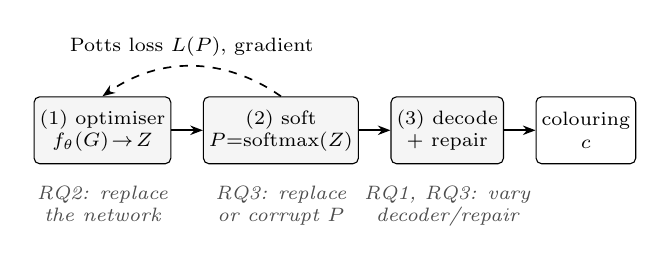
\begin{tikzpicture}[
  font=\scriptsize,
  box/.style={draw, rounded corners=2pt, align=center, minimum height=8.5mm,
              inner sep=2pt, fill=gray!8},
  arr/.style={-{Stealth[length=1.6mm]}, semithick},
  rq/.style={align=center, text=black!70, font=\scriptsize\itshape}]
\node[box] (opt) {(1) optimiser\\$f_\theta(G)\!\to\! Z$};
\node[box, right=4mm of opt] (P) {(2) soft\\$P{=}\mathrm{softmax}(Z)$};
\node[box, right=4mm of P] (dec) {(3) decode\\+ repair};
\node[box, right=4mm of dec, fill=white] (c) {colouring\\$c$};
\draw[arr] (opt) -- (P);
\draw[arr] (P) -- (dec);
\draw[arr] (dec) -- (c);
\draw[arr, dashed] (P.north) to[bend right=35]
  node[above, font=\scriptsize]{Potts loss $L(P)$, gradient} (opt.north);
\node[rq, below=1.5mm of opt] {RQ2: replace\\the network};
\node[rq, below=1.5mm of P] {RQ3: replace\\or corrupt $P$};
\node[rq, below=1.5mm of dec] {RQ1, RQ3: vary\\decoder/repair};
\end{tikzpicture}}
\caption{The three ingredients of PI-GNN colouring and where each research
question intervenes. The graph enters both the network and the loss.}
\label{fig:pipeline}
\end{figure}

The main experiments use $k=\chi(G)-1$ colours. Zero conflicts are then
impossible, so methods are compared on a graded conflict count rather than a
success rate that saturates on easy graphs; a second protocol checks $k=\chi$
and planted random graphs.

Our answer is that \textbf{descent on the Potts loss does the work and noise
decides how well}. Training yields one confident colouring stuck short of a
local optimum (RQ1); the network's edge over free logits is its dropout noise
(RQ2); and decoders find nothing left to decode (RQ3). The protocol itself,
with its uninformative-input and search-start controls, is a second
contribution.\footnote{Code and results:
\url{https://github.com/guretskiysemyon/GraphsML}. Implementation,
experiments and drafting used AI coding assistants extensively; all numbers
come from the accompanying code and results, and the design, interpretation
and final text are our own.}

\section{Background and Related Work}

\paragraph{Learning for combinatorial optimisation.} Learned methods either
construct solutions or guide classical solvers \cite{bengio2021ml4co}. For
colouring, \citet{lemos2019gcp} trained a supervised GNN to decide
$k$-colourability. Unsupervised approaches instead minimise a differentiable
relaxation on each instance. \citet{karalias2020erdos} relax the objective to
an expectation under independent vertex distributions and recover a solution by
derandomised rounding \cite{raghavan1988derandomization}, with a guarantee in
terms of the relaxed loss. PI-GNN \cite{schuetz2022combopt,schuetz2022colouring}
applies the same idea with a QUBO or Potts energy \cite{wu1982potts} and a
GraphSAGE network \cite{hamilton2017sage}, reporting results competitive
with classical solvers on DIMACS graphs \cite{johnson1996dimacs}.

\paragraph{Critiques and ablations.} \citet{angelini2023cautionary} and
\citet{boettcher2023inability} showed, end to end, that simple greedy
algorithms match or beat PI-GNN on maximum independent set and max-cut.
\citet{vanderbush2026nar} include a direct-logit (depth-zero)
ablation of a modified PI-GNN for colouring. We make that comparison the
central object and add what an ablation alone leaves open: a shared start,
separate tuning, matched time, noise controls and a common repair step.

\paragraph{Classical references and training dynamics.} DSATUR
\cite{brelaz1979} colours the most constrained vertex first. TabuCol
\cite{hertz1987tabu} is a local search that accepts worsening moves and
forbids recent reversals, and underlies state-of-the-art hybrids
\cite{galinier1999hybrid}. Two facts about training matter for RQ2: a network moves its output through shared
parameters, so one step moves many vertices at once \cite{jacot2018ntk}, and
dropout \cite{srivastava2014dropout} injects noise into training.

\section{Setup}
\label{sec:method}

\paragraph{Relaxation.} A soft colouring $P\in\mathbb{R}^{n\times k}$ has one
probability row $p_v$ per vertex, obtained from logits by
$P=\mathrm{softmax}(Z)$. The Potts loss and the hard conflict count are
\begin{align*}
L(P)&=\textstyle\sum_{\{u,v\}\in E}p_u^{\top}p_v,\\
C(c)&=\textstyle\sum_{\{u,v\}\in E}\mathbf{1}[c_u=c_v].
\end{align*}
Since $p_u^\top p_v$ is the probability that $u$ and $v$ draw the same colour,
$L(P)$ is the expected conflict count when each vertex samples independently,
and $L=C$ when every row is one-hot.

\paragraph{Local optimality and repair.} Let $M_v(a)$ be the number of
neighbours of $v$ with colour $a$. Recolouring $v$ can remove at most
$\gamma_v=M_v(c_v)-\min_a M_v(a)$ conflicts, and a colouring is
\emph{single-flip optimal} (SFO) when $\gamma_v=0$ for all $v$. Our shared
repair, \emph{strict descent}, repeatedly applies a move with the largest
positive $\gamma_v$ and stops at an SFO colouring. We report raw conflicts $C$
(how good a method's own answer is) and $\Cd$ after descent (how good a
\emph{starting point} it is); in RQ2 the two disagree.

\begin{lemma}[cf.\ \citealp{rosenberg1972}]\label{lem:strict}
If $P^*$ is a strict local minimum of $L$ over all row-stochastic matrices,
every row is one-hot and every single-vertex recolouring strictly increases $C$.
\end{lemma}

\noindent The proof (Appendix~\ref{app:proof}) rests on $L$ being affine in
each row: with other rows fixed, $L=B+p_v^\top q_v$ with
$q_v=\sum_{u\in N(v)}p_u$. Training, however, moves logits rather than
probabilities, and for the Potts loss
\begin{equation}
\frac{\partial L}{\partial z_{v,a}}=p_v(a)\bigl[q_v(a)-p_v^\top q_v\bigr].
\label{eq:grad}
\end{equation}
Suppose $p_v$ is nearly one-hot on colour $c$. For $a\neq c$ the factor
$p_v(a)\approx e^{-\Delta}$ is tiny, where $\Delta$ is the gap between the top
two logits; for $a=c$ the bracket is $\approx q_v(c)-q_v(c)=0$. So every logit
gradient of a \emph{saturated} vertex vanishes, even when another colour would
remove many conflicts.

\paragraph{PI-GNN and benchmark.} We reimplement PI-GNN in PyTorch: trainable
Gaussian vertex embeddings (dimension 85), two mean-aggregation GraphSAGE
layers (hidden width 30, ReLU, dropout $0.47$), trained full-batch with AdamW
\cite{loshchilov2019adamw}. The benchmark is the 68 DIMACS graphs whose
chromatic number is proven \cite{held2012safe,gualandi2012exact}, with 11 to
1{,}000 vertices from 14 families: 5 seeds per graph, $10^5$ steps, no early
stopping, dropout off at evaluation. Every model type is
tuned separately by the same two-stage random search on 13 disjoint synthetic
graphs, then frozen.

\paragraph{Second protocol.} Independent runs at $k=\chi$ check the same
questions on the 12 DIMACS graphs of \citet{schuetz2022colouring}, 12 harder
ones, and 27 planted 5-colourable random graphs near the clustering threshold
\citep{zdeborova2007phase}, pairing runs by graph and seed; ties are exact.

\paragraph{Comparison rule.} The graph is the unit of analysis: we average
the 5 seeds per graph and compare paired means $X_g,Y_g$ through
$d_g=(X_g-Y_g)/\max(Y_g,1)$. A graph is a practical tie if $|X_g-Y_g|<1$
conflict or $|d_g|\le 5\%$, otherwise a win or a loss. We report
wins/ties/losses (W/T/L), the median $d_g$ and a two-sided Wilcoxon
signed-rank test \cite{wilcoxon1945}. A directional claim needs a small $p$
(Bonferroni-corrected over the primary comparisons), a median beyond $5\%$
and more wins than losses; anything else is ``not
distinguishable'', which is not a claim of equality. The rule was fixed before
the main RQ2 results were computed; it rests on medians because conflict
counts span four orders of magnitude.

\section{Experiments}

\subsection{RQ1: Sure but stuck}

\emph{What does training produce?} One confident colouring, usually short of a
local optimum. Figure~\ref{fig:rq1} tracks the argmax output over training.
The fraction of SFO runs rises from $0\%$ to $42\%$ ($143/340$), and the
median share of conflicts that descent can still remove falls from $95\%$ to
$10\%$. Both curves flatten after $5{\cdot}10^4$ steps. Extending 13
still-improving graphs to $3{\cdot}10^5$ steps lowers conflicts after descent
on 12, yet SFO runs go from $0/65$ to only $1/65$. Longer training finds
better basins without reaching their bottoms: it delivers the one-hot rows of
Lemma~\ref{lem:strict}, not its local optimality.

\begin{figure}[t]
\centering
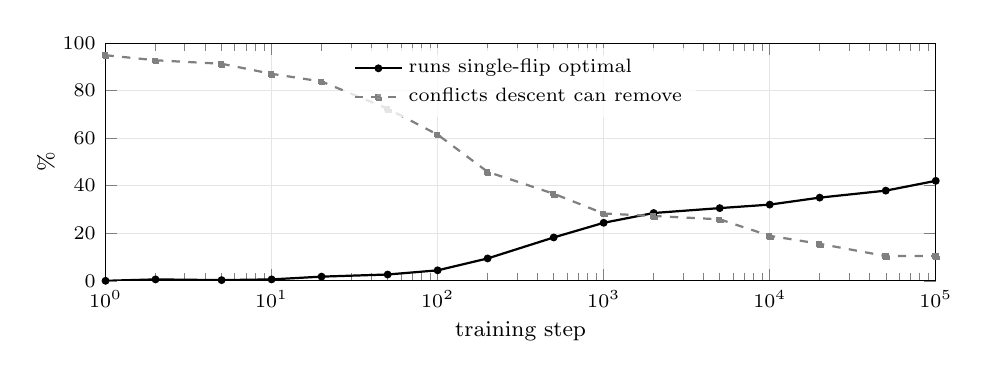
\begin{tikzpicture}
\begin{axis}[
  width=\columnwidth, height=4.6cm,
  xmode=log, xmin=1, xmax=100000,
  ymin=0, ymax=100,
  xlabel={training step}, ylabel={\%},
  xlabel style={font=\footnotesize, yshift=2pt},
  ylabel style={font=\footnotesize, yshift=-4pt},
  tick label style={font=\scriptsize},
  legend style={font=\scriptsize, at={(0.5,0.98)}, anchor=north,
                draw=none, fill=white, fill opacity=0.8, text opacity=1},
  legend cell align=left, grid=major, grid style={gray!20}]
\addplot[thick, black, mark=*, mark size=1pt] coordinates {
 (1,0.0) (2,0.59) (5,0.29) (10,0.59) (20,1.76) (50,2.65) (100,4.41)
 (200,9.41) (500,18.24) (1000,24.41) (2000,28.53) (5000,30.59)
 (10000,32.06) (20000,35.0) (50000,37.94) (100000,42.06)};
\addlegendentry{runs single-flip optimal}
\addplot[thick, gray, dashed, mark=square*, mark size=1pt] coordinates {
 (1,94.92) (2,92.79) (5,91.32) (10,87.09) (20,83.86) (50,72.43) (100,61.51)
 (200,45.86) (500,36.64) (1000,28.32) (2000,27.28) (5000,25.86)
 (10000,18.93) (20000,15.57) (50000,10.41) (100000,10.47)};
\addlegendentry{conflicts descent can remove}
\end{axis}
\end{tikzpicture}
\caption{RQ1: PI-GNN's argmax output over training (68 graphs, 5 seeds).
Solid: share of runs single-flip optimal. Dashed: median relative conflict
reduction strict descent still achieves.}
\label{fig:rq1}
\end{figure}

The remaining errors sit on a handful of vertices (median $2.5$ improvable
vertices per run, under $1\%$ of the graph), and those vertices are
\emph{confident}. In the median graph, $99.7\%$ of vertices have
$\max_a p_v(a)\ge 0.99$, and so do $100\%$ of the improvable ones; their median
top-two logit gap is about $150$, so the better colour has probability
$\approx e^{-150}$. The ``distribution'' is a single colouring. By
Eq.~\eqref{eq:grad}, a confident
wrong vertex gets almost no gradient towards the better colour: one flip away,
yet out of reach. This is a plausible mechanism, not a proven one, since shared
parameters can still move such a vertex indirectly.

Is the endpoint at least good? Table~\ref{tab:rq1} compares PI-GNN after
descent with references given the same descent. Training clearly beats random
and epoch-1 starts, but it is not distinguishable from DSATUR, a 1979 greedy
heuristic, and a time-matched TabuCol finds fewer conflicts on 41 graphs. The
queen family makes the point sharply: $85\%$ of queen runs are already SFO,
yet TabuCol wins on all 12 queen graphs. A local minimum can be shallow.

\begin{table}[t]
\centering\small
\begin{tabular}{@{}lcr@{}}
\toprule
PI-GNN + descent vs.\ & W/T/L & median $d$ \\
\midrule
random colouring + descent & \wtl{62}{5}{1} & $-38.7\%$ \\
own epoch-1 output + descent & \wtl{59}{8}{1} & $-32.5\%$ \\
DSATUR + descent & \wtl{16}{28}{24} & $0.0\%$ \\
TabuCol, time-matched & \wtl{14}{13}{41} & -- \\
\bottomrule
\end{tabular}
\caption{RQ1: quality of the trained endpoint at $10^5$ steps, counted from
PI-GNN's side (negative $d$ favours PI-GNN). Mean conflicts: PI-GNN $114.9$,
TabuCol $70.5$.}
\label{tab:rq1}
\end{table}

\subsection{RQ2: Noise in disguise}

\emph{Is the network needed?} Only as a source of noise. The graph already
enters the Potts loss, so a network is not needed to ``use'' it. The natural
network-free competitor, arm B, optimises the logit matrix $Z$ directly from
PI-GNN's exact initial output, so only the optimisation differs.
The other arms each change one thing (Table~\ref{tab:rq2}); two need a word.
B-noise adds Gaussian noise of a preset scale $\sigma$ to $Z$ during
training, reusing B's tuning. D is PI-GNN linearised at initialisation, $Z=Z_0+J_0\delta$ with a
frozen Jacobian, which tests whether the network acts as a fixed
graph-dependent preconditioner.

\begin{table*}[t]
\centering\small\setlength{\tabcolsep}{4pt}
\begin{tabular}{@{}llcccrrr@{}}
\toprule
& & \multicolumn{3}{c}{vs.\ A, W/T/L (arm better / tie / A better)} & & & \\
\cmidrule(lr){3-5}
Arm & change relative to A & raw $C$ & after descent & median $d$ (desc.) &
mean $\Cd$ & SFO & logit gap \\
\midrule
A & PI-GNN (reference) & -- & -- & -- & 114.9 & 42\% & 204 \\
B & free logits from A's start & \wtl{32}{23}{13} & \wtl{17}{25}{26} & $+6.0\%$ & 108.6 & 100\% & 18 \\
B-rand & as B, random start & \wtl{28}{21}{19} & \wtl{20}{20}{28} & $+10.8\%$ & 107.1 & 100\% & 19 \\
A-no-drop & dropout removed & \wtl{10}{9}{49} & \wtl{7}{40}{21} & $+8.7\%$ & 115.7 & 17\% & 18 \\
B-noise-0.5 & B + logit noise, $\sigma{=}0.5$ & \wtl{33}{21}{14} & \wtl{20}{19}{29} & $+5.8\%$ & 109.2 & 100\% & 19 \\
B-noise-1 & B + logit noise, $\sigma{=}1$ & \wtl{46}{20}{2} & \wtl{35}{30}{3} & $-15.9\%$ & 92.5 & 100\% & 13 \\
B-noise-2 & B + logit noise, $\sigma{=}2$ & \wtl{53}{13}{2} & \wtl{44}{21}{3} & $-27.5\%$ & 83.4 & 100\% & 8 \\
C & node MLP: aggregation removed & \wtl{20}{28}{20} & \wtl{5}{35}{28} & $+7.8\%$ & 120.4 & 41\% & 139 \\
D & linearised at init, frozen $J_0$ & \wtl{14}{12}{42} & \wtl{0}{10}{58} & $+36.6\%$ & 130.4 & 42\% & 23 \\
\bottomrule
\end{tabular}
\caption{RQ2 at $10^5$ steps (68 graphs, 5 seeds). W/T/L and median
$d=(\text{arm}-\text{A})/\max(\text{A},1)$ are graph-level; negative $d$
favours the arm. SFO: share of runs single-flip optimal. Logit gap: median
top-two logit difference (saturation). B vs.\ A is the primary comparison.}
\label{tab:rq2}
\end{table*}

\paragraph{The verdict flips with repair.} Free logits give \emph{better raw}
colourings than PI-GNN (32 wins, 13 losses, $p=0.002$). After descent, PI-GNN
is better (26 wins, 17 losses, median $6\%$, $p<0.001$), also at matched
wall-clock time, where B gets about $2.9\times$ more steps. The SFO column explains why: B ends single-flip optimal in all
340 runs, so descent adds nothing to it, while PI-GNN stops short in $58\%$ of
runs but in slightly deeper basins. By the \emph{mean}, B
is still lower (108.6 vs.\ 114.9), as PI-GNN's wins come on low-conflict
graphs.

\paragraph{The advantage is noise, not architecture.} Remove dropout and
PI-GNN's edge is gone: A-no-drop loses to PI-GNN on 21 graphs (7 wins) and is
not distinguishable from B after descent (and in a second-protocol pilot,
dropout won all 8 matched learning-rate and width pairs). Add noise to free
logits and the edge is overturned: after descent
they beat PI-GNN on 35 graphs at $\sigma=1$ and on 44 at $\sigma=2$, losing on
3, and at $\sigma=2$ beat plain B on 53 graphs with no losses. Mean conflicts
(Tables~\ref{tab:rq1}--\ref{tab:rq2}) read as a ladder: network 114.9, free
logits 108.6, with noise 92.5 and 83.4, time-matched TabuCol 70.5.

\paragraph{Dropout and logit noise reshape confidence differently.} Dropout
delays PI-GNN's commitment (69\% of vertices confident at step 100 vs.\ 89\%
without it) but ends far more saturated (median logit gap 204 vs.\ 18). Logit
noise at $\sigma=2$ commits earlier (82\% vs.\ 55\% at step 1k) yet stops
sharpening (93\% confident vs.\ 100\%, gap 8 vs.\ 18 for plain B). So the best
arm keeps some uncertainty late, as a temperature would
\citep{kirkpatrick1983annealing,peterson1989potts}, while dropout pushes
outputs into the saturated regime of Eq.~\ref{eq:grad}; this link to quality
is correlational, not causal.

\paragraph{What does the network contribute?} Aggregation helps only within
the neural recipe: the node MLP C ties PI-GNN on raw colourings (20/28/20) but
loses after descent (5/35/28). D, with its Jacobian frozen at initialisation,
never beats PI-GNN after descent (0/10/58), and B ties B-rand (14/42/12): the
initial output gives no head start.

\begin{table}[t]
\centering\small
\begin{tabular}{@{}lcr@{}}
\toprule
first vs.\ second & W/T/L & median $d$ \\
\midrule
trained vs.\ colour-scrambled & \wtl{48}{20}{0} & $-25.5\%$ \\
trained vs.\ vertex-shuffled & \wtl{56}{12}{0} & $-29.9\%$ \\
trained vs.\ untrained & \wtl{51}{14}{3} & $-22.2\%$ \\
trained vs.\ near-uniform & \wtl{27}{28}{13} & $0.0\%$ \\
\midrule
D-CE vs.\ argmax, raw & \wtl{33}{35}{0} & $-11.4\%$ \\
D-CE vs.\ argmax, after descent & \wtl{22}{46}{0} & $-2.8\%$ \\
\midrule
\multicolumn{3}{@{}l}{\emph{Second protocol (runs paired)}} \\
trained vs.\ DSATUR best of 11 & \wtl{15}{27}{12} & -- \\
D-CE vs.\ argmax, repaired, planted & \wtl{2}{22}{3} & -- \\
TabuCol: trained vs.\ random start & \wtl{22}{22}{22} & -- \\
\quad same, planted graphs & \wtl{13}{0}{14} & -- \\
\bottomrule
\end{tabular}
\caption{RQ3 controls. Top: D-CE + descent on frozen $10^5$-step outputs;
``trained'' is PI-GNN's $P$ unless stated. Bottom: one D-CE decode at $k=\chi$
(also $\chi+1$ for TabuCol on the harder graphs), unrepaired unless marked.}
\label{tab:rq3}
\end{table}

\subsection{RQ3: Nothing left to decode}

\emph{Is it the soft output or the decoder?} Neither adds much to the
colouring that $P$ already encodes. We fix the decoder and vary its input.
The decoder is derandomised conditional expectation (D-CE)
\cite{raghavan1988derandomization,karalias2020erdos}: it fixes vertices in
DSATUR order, giving $v$ the colour $a$ that minimises the number of fixed
neighbours coloured $a$ plus $\sum p_u(a)$ over unfixed neighbours $u$. This
guarantees $C\le L(P)$, but on a one-hot $P$, where $L=C$, it only promises to
match argmax. The first term reads the graph, so D-CE needs no learned
information: on uniform $P$ it is DSATUR, and on near-uniform $P$ it beats raw
argmax on all 68 graphs (median $-93\%$). This near-uniform input is
our \emph{graph-only} baseline. We also corrupt the trained $P$ in three ways:
the untrained output, rows shuffled across vertices, and colours permuted
independently within each row (same confidence, no neighbour agreement).

\paragraph{Real information, but no more than the graph alone.} Trained $P$
beats all three corruptions (Table~\ref{tab:rq3}; medians $-22$ to $-30\%$, at
most 3 losses), including colour-scrambled $P$ with identical confidence, so
its useful content is \emph{coordination} between neighbours, not confidence. Against the graph-only baseline, however, trained $P$ is not
distinguishable (27/28/13, median $0\%$, $p=0.23$), echoing RQ1's tie with
DSATUR. Scrambled $P$ is worse than no $P$ at all (near-uniform wins 41/24/3),
which is why beating a corruption is a weak test. The tie hides a family
split (see Limitations).

\paragraph{Most of the decoder's gain is repair.} On trained $P$, D-CE beats
raw argmax (33/35/0, median $-11.4\%$). Once argmax also gets descent, the gain
shrinks to $-2.8\%$ (22/46/0): inside the tie band, though never worse and
cheaper overall (21 vs.\ 30\,s). Best-of-32 sampling adds nothing (2/65/1) at
$26\times$ the cost, presumably because saturated rows make samples largely
repeat argmax. The second protocol agrees (Table~\ref{tab:rq3}, bottom), and
TabuCol does as well from a random start as from the trained colouring:
whatever $P$ knows, local search rebuilds within $10^4$ iterations.

\paragraph{The optimiser still decides.} Decoding all nine RQ2 arms with D-CE
narrows their spread (median within-graph range $-10\%$) but keeps their
order: B-noise-2 still beats PI-GNN (35/29/4), D stays last, and only
B-noise-2's $P$ beats the graph-only baseline (36/27/5). A better optimiser
gives a better $P$, and decoding keeps that edge.

\section{Discussion and Conclusion}

Returning to Figure~\ref{fig:pipeline}: the optimiser earns the credit
through its noise, not its architecture; the soft output carries real
coordination, but no more than the graph alone; and the decoder's gain is
mostly repair. Descent on the Potts loss does the work, noise decides how well,
and the best gradient-based procedure we found has no network at all. This
sharpens the end-to-end critiques
\cite{angelini2023cautionary,boettcher2023inability}: PI-GNN learns
coordinated structure but commits and saturates before local optimality
(Eq.~\ref{eq:grad}), and what helps it, noise, is cheaper without a network.

For evaluating such methods we suggest, following fair-comparison work
\citep{errica2020fair,bechlerspeicher2025position}: report raw \emph{and}
repaired quality, and whether the output is still a distribution; start a
local search from it and from a random colouring;
use free logits as the network-free baseline; test learned outputs against an
uninformative input under the same decoder; and report per-family results.

Confidence, local optimality and quality are three different things, and
conflating them overstates what the network contributes. Natural next steps
are tuned noisy logit optimisation against strong local search and, where
instances hide global structure, convex relaxations
(Appendix~\ref{app:sdp}).

\section*{Limitations}

One architecture, one main regime ($k=\chi-1$) and 68 heterogeneous graphs
limit generality, and behaviour differs by family: the RQ3 tie hides trained
$P$ winning on all 12 queen graphs but losing on 5/12 Leighton, 2/3 DSJR, 3/5
miles and 3/6 fpsol/inithx graphs, and decoders do matter where training
collapses (one queen13\_13 run: 3{,}328 to 72 conflicts under D-CE). The
second protocol uses published settings and run-level statistics, so across
protocols we compare directions, not magnitudes; on its planted graphs the
repaired trained colouring beats DSATUR's best of 11 (22/2/3), but one second
of TabuCol reaches 13.4 conflicts.
The three noise scales were fixed in advance, not tuned; noisy free logits
were not compared with TabuCol; A-no-drop reuses A's settings; and logit
noise and dropout differ, so reading dropout as noise is supported but not
isolated. The annealed-penalty schedule we tried
\citep{ichikawa2024controlling} did not help, inference-time noise
\citep{colantonio2024efficient} is untested, and Appendix~\ref{app:sdp} rests
on 12 graphs and 2 seeds. $p$-values are descriptive; bootstrap intervals are
in the supplementary appendix.

\bibliography{custom}
\bibliographystyle{acl_natbib}

\clearpage
\onecolumn
\raggedbottom
\appendix
\renewcommand{\thetable}{\thesection.\arabic{table}}
\setcounter{table}{0}

\section{Further effort: domain knowledge from a convex relaxation}
\label{app:sdp}

\paragraph{Motivation.} The Potts loss has no relaxation gap: its continuous
minimum equals the discrete one \citep{rosenberg1972}, so descending it adds no
information beyond what local moves can find. Colouring has a classical
relaxation that does carry global information, vector colouring by
semidefinite programming \citep{karger1998sdp}. We use the Frieze--Jerrum form
at $k$ colours \citep{frieze1997maxkcut}: unit vectors $v_i$ whose pairwise
inner products are at least $-1/(k-1)$, the value between the vertices of a
regular simplex, maximising $\sum_{\{u,v\}\in E}(1-v_u^{\top}v_v)$. A proper
$k$-colouring placed on the simplex puts every edge exactly at this floor. The
problem is convex; we solve it approximately with a rank-32 Burer--Monteiro
factorisation \citep{burer2003nonlinear}, in 11--132\,s per graph on one CPU.

\paragraph{Two uses.} (i)~As domain-informed input to PI-GNN: the vectors
initialise its vertex embeddings (\emph{FJ init}). (ii)~Alone: k-means on the
vectors gives a colouring, which can also seed TabuCol. We ran both on the 12
harder DIMACS graphs of the second protocol (Section~\ref{sec:method}; 2
seeds), against PI-GNN with the best setting of a small pilot, DSATUR and
TabuCol (Table~\ref{tab:sdp}).

\begin{table}[htbp]
\centering\small
\begin{tabular}{@{}lrrrrr@{}}
\toprule
graph ($k$) & PI-GNN & +FJ init & SDP alone & DSATUR & TabuCol \\
\midrule
DSJC125.5 (17) & 19 & 10 & 31 & 21 & 0 \\
DSJC250.5 (28) & 55.5 & 42 & 50 & 60 & 0.6 \\
flat300\_28\_0 (28) & 110 & 96 & 153 & 124 & 32.2 \\
le450\_15a (15) & 31 & 36.5 & 256 & 7 & 0 \\
le450\_15b (15) & 35 & 32.5 & 238 & 7 & 0 \\
le450\_15c (15) & 223 & \textbf{0} & 2 & 248 & 16.2 \\
le450\_15d (15) & 215.5 & \textbf{0.5} & 8 & 250 & 26.8 \\
queen10\_10 (11) & 10 & 9.5 & 54 & 10 & 0 \\
queen12\_12 (12) & 31 & 26 & 61 & 29 & 9.6 \\
queen14\_14 (14) & 32.5 & 32 & 91 & 32 & 13.4 \\
queen15\_15 (15) & 41.5 & 36 & 94 & 42 & 15.2 \\
queen16\_16 (16) & 43.5 & 46 & 117 & 44 & 17 \\
\bottomrule
\end{tabular}
\caption{Conflicts at $k$ colours (second protocol, mean of 2 seeds). PI-GNN
and +FJ init: best colouring found during training; SDP alone: k-means on the
FJ vectors, best of 5; DSATUR: best of 11 randomised runs; TabuCol: 10\,s, mean
of 5 runs.}
\label{tab:sdp}
\end{table}

\paragraph{Where structure is global, geometry wins.} FJ init improves PI-GNN
on 10 of the 12 graphs. On the Leighton graphs le450\_15c/d, built around a
planted 15-colouring \citep{leighton1979}, it is decisive: 0 and 0.5 conflicts,
where plain PI-GNN keeps over 200 and TabuCol 16--27 after 10\,s (7--24 after
60\,s). The control shows why. 95--97\% of edges sit exactly at the floor, so
the SDP has recovered the planted colouring, and TabuCol started from its
k-means colouring finds a proper colouring within 1--72 iterations (10 of 10
starts). The network is not needed: the geometry carries the solution.

\paragraph{Elsewhere it does not.} On random, queen and the sparser Leighton
graphs (le450\_15a/b), the vectors alone are worse than DSATUR on 9 of 10
graphs (e.g.\ 54 vs.\ 10 conflicts on queen10\_10), FJ init helps PI-GNN
unevenly (most on DSJC125.5, from 19 to 10), and TabuCol stays far ahead.
Earlier small-scale tests agree. In an RLF-style colour-class extraction on 13
small graphs, SDP vectors lowered the mean excess over the best known colour
count from 0.615 (RLF) to 0.385, but random unit vectors in the same procedure
reached 0.462 (3/35/1 SDP vs.\ random). As PI-GNN input features on 9 small
graphs, FJ vectors beat the same rows shuffled (21/3/3) but not identity
features significantly (16/6/5, Holm-corrected $p=0.18$).

\paragraph{Insight.} Domain knowledge from a convex relaxation helps exactly
where an instance hides global structure. There it solves what neither PI-GNN
nor TabuCol can, and the Potts loss, being exact, cannot supply it. Where
hardness lies in a rugged landscape instead, only search helps. Testing all
twelve Leighton graphs and planted-partition models would locate the boundary.

\section{Proof sketch of Lemma~\ref{lem:strict}}
\label{app:proof}

With other rows fixed, $L=B+p_v^\top q_v$ where $q_v=\sum_{u\in N(v)}p_u$, so
$L$ is affine in $p_v$. Moving mass $\epsilon$ between two colours $a,b$ in
the support of $p_v$ changes $L$ by $\pm\epsilon(q_v(a)-q_v(b))$, so one of the
two moves does not increase $L$, contradicting strictness. At a one-hot row,
moving mass $t$ towards colour $a$ changes $L$ by $t\,[M_v(a)-M_v(c_v)]$, which
must be positive.

\end{document}
